% Format teze zasnovan je na paketu memoir
% http://tug.ctan.org/macros/latex/contrib/memoir/memman.pdf ili
% http://texdoc.net/texmf-dist/doc/latex/memoir/memman.pdf
% 
% Prilikom zadavanja klase memoir, navedenim opcijama se podešava 
% veličina slova (12pt) i jednostrano štampanje (oneside).
% Ove parametre možete menjati samo ako pravite nezvanične verzije
% mastera za privatnu upotrebu (na primer, u b5 varijanti ima smisla 
% smanjiti 
\documentclass[12pt,oneside]{memoir}
% Paket koji definiše sve specifičnosti mastera Matematičkog fakulteta
\usepackage{matfmaster}
%
% Podrazumevano pismo je ćirilica.
%   Ako koristite pdflatex, a ne xetex, sav latinički tekst na srpskom jeziku
%   treba biti okružen sa \lat{...} ili \begin{latinica}...\end{latinica}.
%
%
% Opicija [latinica]:
%   ako želite da pišete latiniciom, dodajte opciju "latinica" tj.
%   prethodni paket uključite pomoću: \usepackage[latinica]{matfmaster}.
%   Ako koristite pdflatex, a ne xetex, sav ćirilički tekst treba biti
%   okružen sa \cir{...} ili \begin{cirilica}...\end{cirilica}.
%
% Opcija [biblatex]:
%   ako želite da koristite reference na više jezika i umesto paketa
%   bibtex da koristite BibLaTeX/Biber, dodajte opciju "biblatex" tj.
%   prethodni paket uključite pomoću: \usepackage[biblatex]{matfmaster}
%
% Opcija [b5paper]:
%   ako želite da napravite verziju teze u manjem (b5) formatu, navedite
%   opciju "b5paper", tj. prethodni paket uključite pomoću: 
%   \usepackage[b5paper]{matfmaster}. Tada ima smisla razmisliti o promeni
%   veličine slova (izmenom opcije 12pt na 11pt u \documentclass{memoir}).
%
% Naravno, opcije je moguće kombinovati.
% Npr. \usepackage[b5paper,biblatex]{matfmaster}

% Pomoćni paket koji generiše nasumičan tekst u kojem se javljaju sva slova
% azbuke (nema potrebe koristiti ovo u pravim disertacijama)
% Datoteka sa literaturom u BibTex tj. BibLaTeX/Biber formatu
\usepackage{multirow}
\usepackage{dcolumn}
\usepackage{amsthm}
\usepackage{tabularx}
\usepackage{ltablex} 
\usepackage{lscape}
\usepackage{booktabs}
\usepackage{enumitem}
\usepackage{listings}
\usepackage{amsmath,amssymb,latexsym}
\usepackage[unicode]{hyperref}
\usepackage{subfig}
\hypersetup{colorlinks,citecolor=green,filecolor=green,linkcolor=blue,urlcolor=blue}
\renewcommand{\lstlistingname}{Код}
 
\newtheorem{definic}{Дефиниција}
\bib{master_branislavaz}

% Ime kandidata na srpskom jeziku (u odabranom pismu)
\autor{Бранислава Б. Живковић}
% Naslov teze na srpskom jeziku (u odabranom pismu)
\naslov{Паралелизација статичке верификације софтвера }
% Godina u kojoj je teza predana komisiji
\godina{2016}
% Ime i afilijacija mentora (u odabranom pismu)
\mentor{др Милена \textsc{Вујошевић Јаничић}, доцент\\ Универзитет у Београду, Математички факултет}
% Ime i afilijacija prvog člana komisije (u odabranom pismu)
\komisijaA{др Саша \textsc{Малков}, ванредни професор\\ Универзитет у Београду, Математички факултет}
% Ime i afilijacija drugog člana komisije (u odabranom pismu)
\komisijaB{др Филип \textsc{Марић}, ванредни професор\\ Универзитет у Београду, Математички факултет}
% Ime i afilijacija trećeg člana komisije (opciono)
% \komisijaC{}
% Ime i afilijacija četvrtog člana komisije (opciono)
% \komisijaD{}
% Datum odbrane (obrisati ili iskomentarisati narednu liniju ako datum odbrane nije poznat)
\datumodbrane{ 2016.}

% Apstrakt na srpskom jeziku (u odabranom pismu)
\apstr{%
}

% Ključne reči na srpskom jeziku (u odabranom pismu)
\kljucnereci{паралелизација, верификација, рачунарство}

\begin{document}
% ==============================================================================
% Uvodni deo teze
\frontmatter
% ==============================================================================
% Naslovna strana
\naslovna
% Strana sa podacima o mentoru i članovima komisije
\komisija
% Strana sa posvetom (u odabranom pismu)
\posveta{Брату, мами и тати}
% Strana sa podacima o disertaciji na srpskom jeziku
%\apstrakt
\mainmatter
% Sadržaj teze
\tableofcontents

% ==============================================================================
% Glavni deo teze
% ==============================================================================

% ------------------------------------------------------------------------------
%\chapter{Увод}
% ------------------------------------------------------------------------------



\chapter{Увод} 

Развој и примена нових технологија почиње све више да утиче на друштво. Рачунари су присутни свуда око нас и пружају нам многе погодности и олакшице како у необавезним тако и у пословним активностима. Институције попут банака, здравства, просвете, и других теже да аутоматизују своје процесе коришћењем разних софтверских алата.  
 
 Грешке у софтверу могу имати катастрофалне последице, на пример отказивање медицинског уређаја у току операције или отказивање аутоматског пилота у току лета. Како бисмо предухитрили овакве ситуације, потребно је детаљно и прецизно утврдити исправност развијеног софтвера. 
 
  Испитивање исправности софтвера може бити динамичко и статичко. Статичка верификација софтвера представља најпоузданији начин испитивања исправности програма, уз битно теоријско ограничење, халтинг проблем \cite{halting}. Наиме, није могуће направити алгоритам који потпуно прецизно испитује исправност произвољног програма у коначном времену користећи коначне ресурсе. \\
\subsection{Мотивација}

 Аутоматизовано статичко утврђивање исправности софтвера захтева анализу програмског кода без његовог извшавања, коришћењем техника статичке анализе. Ове технике могу бити веома сложене и захтевне у пољу времена и ресурса, што додатно ограничава сам процес.

 Алати за аутоматску статичку верификацију софтвера због свих поменутих ограничења могу бити веома комплексни, због чега је погодно покретати их на рачунарима са јаким хардверским перформансама. Временом су процесори са више језгара почели да доминирају тржиштем и данас готово сваки нов рачунар садржи вишејезгарни процесор. Такође, рачунари са више процесора постају све доступнији што нам даје могућност да пишемо софтвер који имплементира конкурентно ивршавање и користи сав потенцијал вишепроцесорских и вишејезгарних система.
 
 У оквиру овог рада надограђен је систем за аутоматску верификацију софтвера LAV \cite{mvjphd}. Процес испитивања исправности програма је паралелизован на два нивоа и приказани су експериментални резултати поређења секвенцијалног и паралелног извршавања система LAV као и експериментално поређење са алатом CBMC \cite{cbmc}. Резултати показују да паралелизација може значајно да убрза, а у неким ситуацијама заправо и омогући, ефикасан процес утврђивања исправности програма.

%Испитивање задовољивости логичке формуле је НП-комплетан проблем и један је од најтежих проблема у рачунарству.


\chapter{Верификација софтвера}
	Верификација софтвера представља дисциплину рачунарства која се бави провером и доказивањем исправности програма. Програм је исправан уколико задовољава задату спецификацију, односно уколико за сваки улаз има одговарајуће понашање које је предвиђено спецификацијом. Постоје два основна приступа верификацији, \emph{динамичка} и \emph{статичка} верификација.
  \section{Динамичка верификација}
  Динамичка верификација програма се врши током његовог извршавања. Грешке у програму се покушавају пронаћи исцрпним тестирањем што је и циљ динамичке верификације. Битно је нагласити да тестирањем није могуће доказати исправност програма већ је могуће пронаћи грешке и на тај начин оповргнути претпоставку о исправности програма. 
  
   Да би се програм тестирао потребно је пронаћи одговарајући скуп улазних података помоћу којих се врши тестирање.  С обзиром на то да је простор могућих улаза углавном превелики, није могуће тестирати програм за све могуће улазе. Због тога треба издвојити одговарајући подскуп улазних података који што боље описује спецификацију програма и покрива што већи број случајева. Избор улазних података се углавном врши коришћењем програмског кода и спецификације. 
   
    Постоје две основне методе тестирања, метод \emph{црне} и 
 \emph{беле} кутије.  Методом црне кутије генерисање тестова се врши на основу спецификације програма не узимајући у обзир детаље имплементације. Методом беле кутије тестови се генеришу на основу кода и структуре програма. Такође, постоји и метод сиве кутије који представља мешавину ова два приступа. У зависности од тога шта је потребно тестирати користи се одговарајући метод \cite{testing}. 
  
  
  \section{Статичка верификација}
  \label{statver}
  Статичка верификација програма представља испитивање исправности програма анализом програмског кода, без његовог извршавања. Анализа програмског кода се врши углавном над изворним или објектним кодом. Особине програма и услови исправности се описују одговарајућим формулама изабране математичке теорије. Изграђене формуле се даље анализирају коришћењем стриктних математичких метода. Неодлучивост халтинг проблема нам говори да није могуће испитати да ли је нека наредба програма достижна, па тиме ни да ли је програм потпуно исправан. Због тога се особине програма апроксимирају и описују одлучивим математичким теоријама. Аутоматизоване технике статичке анализе су \emph{проверавање модела}, \emph{апстрактна интерпретација} и \emph{симболичко извршавање}.  
  
Проверавање модела је техника верификације којом се испитује да ли модел програма задовољава одговарајућу спецификацију. Модел програма се описује коначним аутоматом који се састоји од стања и прелаза између стања, а спецификација се описује логичком формулом. Испитивање исправности програма се врши исцрпним и систематским обиласком стања аутомата како би се доказали услови задати спецификацијом. Уколико доказивање није могуће, генерише се одговарајући контрапример \cite{verif_tech}.

Апстрактна интерпретација представља метод верификације код кога се семантика програма апроксимира математичким моделом. Понашање програма се описује одговарајућим апстрактним доменом и релацијама над њиме. Анализом апстрактног домена могуће је добити информације о резултатима рада програма без његовог извршавања \cite{verif_tech}. 

Симболичко извршавање је метод верификације који анализира понашање програма на основу симболичких вредности променљивих. Путање програма се описују симболичким изразима а испитивање исправности програма се врши анализом конструисаних израза. Резултати анализе неке путање програма важе за све могуће улазне вредности променњивих које прате дату путању \cite{symbolic_exec}.

  \section{Алати за верификацију}
У наставку ће бити описани неки верификациони алати који користе поменуте технике приликом испитивања исправности програма. 

\paragraph{ LLBMC (енг. Low-Level Bounded Model Checker)} је алат који проверава исправност 
C и C++ програма. Користи технике за проверавање ограничених модела над LLVM међукодом. Проналази грешке дељења нулом, прекорачење бафера, неисправног и двоструког ослобађања меморије, прекорачења у аритметичким изразима и проверава кориснички задате услове. За проверавање услова исправности користи SMT решаваче STP i Boolector \cite{llbmc}.

\paragraph{KLEE} је алат који врши симболичко извршавање и генерисање тест примера над програмима који су писани у језику C. Настао је на Универзитету Илиноис и јавно је доступан. KLEE анализира LLVM међукод користећи SMT решавач STP приликом испитивања услова исправности \cite{klee}. 

\paragraph{CBMC} је алат за верификацију C и C++ програма првенствено намењен за верификацију уграђених система (енг. embedded systems). CBMC врши симболичко израчунавање тако што изворни код програма претаче у SAT формулу и испитује њену задовољивост \cite{cbmc}. 

  \section{Систем LAV}
	LAV је алат за статичку верификацију софтвера \cite{mvjphd}. Oтвореног је кода и доступан је на адреси \url{http://argo.matf.bg.ac.rs/?content=lav}. 
	
	LAV имплементира статичку анализу, генерисање и испитивање услова исправности императивних програма комбинујући методе описане у поглављу \ref{statver}. Користи LLVM инфраструктуру ради трансформације програма у форму која је погодна за анализу и првенствено је намењен за анализу програма написаних у програмском језику C. Међутим, универзалност LLVM платформе омогућава и анализу других процедуралних језика који се могу компајлирати у LLVM код, као што су језици C++, Ada и Fortran. LAV моделује понашање програма и генерише услове исправности трансформишући их у формуле одговарајуће теорије логике првог реда. Теорије које су подржане су аритметика бит-вектора, линеарна аритметика, теорија неинтерпретираних функција (или акерменизација) и теорија низова.  Симболичким извршавањем LAV генерише формуле изабране теорије логике првог реда које описују понашање сваког блока LLVM међукода као и њихове релације. 
	
	LAV генерише формуле исправности неке наредбе и испитује њихову задовољивост користећи SMT решавач. Комбинацијом ових формула граде се формуле које описују понашање програма. 
	
	 Формуле се конструишу по потреби у различитим контекстима. Контекст дефинише информације из околине наредбе које ће бити узете у разматрање приликом расуђивања о наредби. Контексти који постоје су празан контекст, контекст блока, контекст функције и контекст у коме је функција позвана. Разликују се по ширини од најужег до најширег. Приликом испитивања исправности наредбе почиње се са празним контекстом.  Након генерисања формуле у оквиру једног контекста, формула се шаље SMT решавачу на проверу. У зависности од резултата испитују се и шири контексти. 
	 
 На основу резултата решавача LAV генерише извештај о безбедности наредби програма \cite{mvjdev}. 	
	 
	
\chapter{Основе паралелизације}
	Термини паралелизам и конкурентност у рачунарству су углавном испреплетани и погрешно схваћени. Често се грешком поистовећују и сматрају синонимима иако то нису. Због тога је битно да их правилно дефинишемо и разликујемо \cite{par_computing}.
%\begin{definic}
%	Конкурентност је својство програма које се односи на то да два или више задатака могу бити истовремено у току. (исправити превод)
%\end{definic}
%\begin{definic}
%	Паралелизам је својство програма да извршава два или више задатака истовремено. (исправити превод)
%\end{definic}

\begin{definic}
	За процесе Т1 и Т2 кажемо да се извршавају конкурентно ако није унапред позната њихова међусобна временска лоцираност.
\end{definic}
\begin{definic}
	Два процеса се извршавају паралелно ако постоји период времена у коме су оба процеса истовремено активни
\end{definic}

Битно је напоменути да постоји разлика у томе да ли се два задатка истовремено извршавају или су истовремено у току. Наиме, паралелизам захтева конкурентност, док обрнуто не важи. Може се рећи да је конкурентност начин структуирања програма, а паралелизам начин извршавања програма. Конкурентни програми се могу извршавати паралелно али не морају. Паралелизам захтева архитектуру која има више процесорских јединица, док се конкурентност може остварити и на једном процесору.

 	Паралелно програмирање је област рачунарства која се бави архитектуром система и софтверским проблемима програма са паралелним извршавањем. Програм се може дефинисати као низ наредби које се извршавају након његовог покретања. Секвенцијалне програме одликује серијско извршавање наредби. Паралелизам је карактеристика програма која се односи на независност његових израчунавања. Независна израчунавања се могу истовремено односно паралелно извршавати на више процесорских јединица.
  \section{Мотивација}
  Интересовање за паралелизацију се јавља касних 1950-их са зачетком теоријских основа док се први технички напредак осећа почетком 1960-их и и даље расте. Први суперрачунари су се појавили 60-их година и имали су више процесора који су могли паралелно да раде са дељеном меморијом. Даљим развојем 80-их година се појављују кластери, системи који се састоје од великог броја рачунара тзв. чворова међусобно повезаних преко мреже. 90-их година са експанзијом интернета се појављује рачунарство у облаку, док данас већина кућних рачунара садржи процесоре са више језгара. 
  
   Може се рећи да перформансе рачунара експоненцијално расту од 1945 године за фактор 10 сваких 5 година. Први рачунари су израчунавали десетине операција са бројевима у покретном зарезу у секунди, паралелни рачунари 1990-их достижу број од пар десетина милијарди операција у секунди. Рачунарске архитектуре су морале да испрате овакав нагли раст што се постиже преласком са секвенцијалног на паралелно програмирање \cite{par_history}.
   
    Перформансе софтверских решења зависе од времена извршавања основних операција, попут операција са бројевима у покретном зарезу, као и од броја оваквих операција које се могу извршавати паралелно. С обзиром на то да ово време зависи од брзине откуцаја часовника процесора која полако тежи ка теоријском максимуму (брзина светлости) не можемо се ослонити на то да ће бржи процесори подићи перформансе нумеричких израчунавања. Главна мотивација и циљ паралелног програмирања је подизање перформанси рачунарских система односно убрзање програма. Потреба за паралелним приступом расте и због тога што је секвенцијалним приступом решавање многих комплексних проблема временски захтевно.
    
     \emph{Убрзање паралелизацијом} је мера која показује колико пута паралелни програми брже решавају исте проблеме него секвенцијални програми. Формула убрзања је следећа \cite{par_various}:
 	$$ S = T_s/T_p $$
 	
\noindent где $ T_s $ представља време извршавања секвенцијаног а $ T_p $ време извршавања паралелног програма за исти проблем. 

 По Амдаловом закону, извршавање паралелног програма на паралелном рачунару углавном обухвата и део операција које се не могу извршавати паралелно. Означимо са $ \alpha $ део програма који се мора извршавати секвенцијално на једном процесору, а остатак $ (1 - \alpha)$ се може извршити паралелно. Ако је $ N $ број процесорских јединица, формула убрзања је: 
 	$$ S = 1 / ( \alpha + (1-\alpha)/N)$$
Ова формула нам показује да убрзање никада не може прећи $ 1/\alpha $, тј. број процесорских јединица не утиче на део програма који се мора извршавати секвенцијално. На слици \ref{fig:amdal} је приказана зависност убрзања од броја процесора и дела посла који се мора обавити секвенцијално.

 \begin{figure}[!ht]
  \centering
  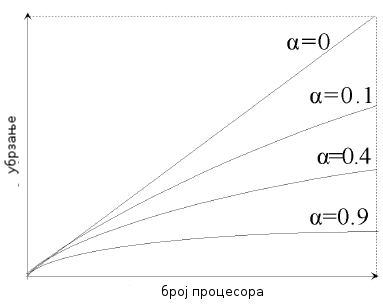
\includegraphics[width=0.8\textwidth]{img/amdal.png}
  \caption{Зависност убрзања од броја процесора за неке вредности $ \alpha $ }
  \label{fig:amdal}
\end{figure}



 У пракси, време извршавања програма на паралелним системима је углавном веће од теоријски израчунате вредности јер зависи и од других параметара попут комуникације и синхронизације. Амдалов модел не узима у обзир ова времена и разматра само случајеве у којима је димензија проблема фиксирана. Поред Амдаловог модела постоје и други модели као што су Густафсонов, Гинтеров, модел Сун Ни-ја који превазилазе нека ограничења Амдаловог модела \cite{performance}.
 	 


  \section{Врсте паралелизације}
  
 Програми се могу паралелизовати на различите начине. Паралелзацију може обављати програмер експлицитно или коришћењем неких алата. Последњих година развијени су многи алати који омогућују аутоматску паралелизацију. Коришћењем ових алата програмеру је олакшан процес паралелизације уз ограничену контролу. Овакав начин паралелизације је погодан за велике и комплексне системе код којих би ручна паралелизација била спора и компликована.
 
  Са друге стране, ручна паралелизација програма захтева добро обучене програмере и углавном је сложенија али пружа програмерима потпуну контролу над самим процесом паралелизације. Овакав приступ је погоднији за паралелизацију специфичних проблема.


  Битно је нагласити да није могуће паралелизовати све делове сваког алгоритма. Посао програмера је да пронађе и одлучи који делови алгоритма се могу паралелизовати и на који начин.
 Два најчешћа приступа дизајнирању паралелних алгоритама су \emph{паралелизација задатака} и \emph{паралелизација података}. 
Паралелизација задатака представља раслојавање алгоритма на независне задатке који се могу извршавати било којим редоследом над истим скупом података.
Паралелизација података представља раслојавање података тако да се један задатак може независно извршавати над дисјунктним деловима података било којим редоследом \cite{art_conc}. 
На слици  \ref{fig:data_parallel} је приказан пример паралелизације задатака а на слици \ref{fig:task_parallel} пример паралелизације података

\begin{figure}[!ht]
  \centering
  \includegraphics[width=0.6\textwidth]{img/data_parallel.png}
  \caption{Пример паралелизације података: примена функције capslock над сваким словом појединачно}
  \label{fig:data_parallel}
\end{figure}

\begin{figure}[!ht]
  \centering
  \includegraphics[width=0.6\textwidth]{img/task_parallel.png}
  \caption{Пример паралелизације задатака: примена различитих функција над свим подацима}
  \label{fig:task_parallel}
\end{figure}


  \section{Изазови процеса паралелизације}
  Често није могуће раслојити алгоритам на потпуно независне задатке који се могу паралелно извршавати већ је присутан одређен ниво зависности између њих. На пример, уколико задаци могу приступити истој променљивој у програму и променити њену вредност, потенцијално више задатака може истовремено покушати да је измени. У таквим ситуацијама задаци се надмећу за приступ дењеним подацима.  Овакви и овоме слични проблеми индукују постојање \emph{критичне секције}. Критична секција представља низ наредби који мора задовољавати следећи услов: уколико је један задатак ушао у критичну секцију и почео да је извршава, ниједан други задатак је не сме извршавати истовремено. У складу са тиме постоје бројна решења и механизми који омогућавају \emph{комуникацију} и  \emph{синхронизацију} између задатака.
  
  
Комуникација представља било који вид размене информација између задатака. Може се остварити преко дељене меморије или слањем односно примањем порука. Комуникација преко порука се одвија тако што један задатак експлицитно шаље податке другом задатку који их прихвата и обрађује. Неки од познатих механизама за овакав вид комуникације су сигнали, цеви, сокети и канали.
Постојање дељене меморије има своје добре и лоше стране. Понекад је потребно старати се о редоследу читања односно писања дељене меморије као и о евентуалним утркивањима и сукобима. Због тога комуникација преко дељене меморије може захтевати одређен ниво синхронизације. Кроз механизме синхронизације програмер може контролисати редослед извршавања задатака и приступ дељеној меморији. Две основне врсте овакве синхронизације су \emph{сарадња} и \emph{такмичење}. Синхронизација сарадње између два задатка је потребна уколико један задатак зависи од резултата рада другог. Синхронизација такмичења је неоходна у случајевима када два задатка истовремено захтевају исти ресурс. Механизми који се користе за имплементацију синхронизације су мутекси, катанци, семафори, монитори и други \cite{lang_prag}.

 Синхронизација отвара многе проблеме, нпр. могућност \emph{узајамног блокирања}, \emph{живог блокирања} и \emph{изгладњивања} између задатака. Ови проблеми се односе на концепт \emph{напредовања} (енг. liveness) програма. Концепт напредовања програма представља својство програма да у току свог извршавања напредује доводећи до предвиђеног догађаја у неком тренутку, односно да константно прави прогрес током свог извршавања. Уколико ово својство није задовољено може да се деси да програм не може да настави са својим извршавањем. Узајамно блокирање (енг. deadlock) се дешава у ситуацији када два задатка чекају један на другог како би наставили са радом и на тај начин губе напредак. Живо блокирање (енг. livelock) представља ситуацију када сви задаци раде али нема напретка. Изгладњивање се односи на могућност да један задатак спречава извршавање другог. Поменути проблеми се могу спречити одговарајућим алгоритмима \cite{opsis}.


 % \section{Неки патерни}
  \section{Библиотеке за паралелизацију}
	У овом поглављу ће бити описане неке библиотеке које се користе за паралелизацију програмског кода. Акценат ће бити на библиотекама за језик C++. 
	
 Алате за паралелизацију можемо поделити у две категорије имплицитне и експлицитне. Имплицитни алати олакшавају програмеру имплементацију паралелних алгоритама јер се старају о прављењу, управљању и синхронизацији нити. Експлицитни алати пружају већу флексибилности и контролу захтевајући од програмера да управља свим аспектима вишенитности.
	
\paragraph{ PThreads (енг. POSIX Threading interface)} је интерфејс за паралелно програмирање на нивоу оперативног система и доступан је у оквиру већине UNIX-оликих оперативних система. Имплементиран је у оквиру заглавља \\ \texttt{pthread.h} језика C који садржи скуп константи, типова и функција за паралелизацију. Програмеру је омогућено прављење нити и управљање њиховим извршавањем. Комуникација се обавља преко дељене меморије коју такође програмер контролише. Дељена меморија се имплементира коришћењем глобалних променљивих које су видљиве свим нитима. Садржај заглавља \texttt{pthread.h} уз одговарајућу документацију се може наћи на адреси \url{http://man7.org/linux/man-pages/man7/pthreads.7.html}.

\paragraph{OpenMP (енг. Open Specification for Multi-Processing)} је интерфејс за програмирање који омогућава паралелно програмирање у језицима C, C++ и Фортран . Заснива се на моделу паралелизације коришћењем дељене меморије. Садржи скуп компајлерских директива, рутина и глобалних променљивих које служе за обележавање делова програмског кода. Програм се дели на регионе који се извршавају серијски и регионе који се извршавају паралелно. Региони се означавају директивама које управљају процесом додељивања задатака нитима, комуникацијом и синхронизацијом. Променљиве могу бити дељене, односно видљиве свим нитима, и приватне, односно видљиве у оквиру нити унутар које су декларисане. Детаљна документација се може наћи на адреси \url{http://www.openmp.org}. 

\paragraph{TBB (енг. Thread Building Blocks)} је C++ библиотека за паралелно програмирање на вишепроцесорским системима развијена од стране \emph{Intel}-а. Библиотека се састоји од бројних шаблона који имплементирају паралелне алгоритме, контејнере, примитиве за синхронизацију и управљач задацима. Програмери дефинишу задатке који ће се извршавати паралелно након чега се управљач задацима стара о току извршавања и техничким детаљима. Више о овој библиотеци се може наћи на адреси \url{http://www.threadingbuildingblocks.org}.


  
\chapter{Модул за паралелизацију}

Mодул који се бави паралелизацијом је развијен у складу са специфичним захтевима система LAV. Систем LAV је сложен верификациони алат писан у C++ језику. Као такав користи многе спољне библиотеке, алате, као и SMT решаваче.  Архитектура самог система је модуларна, функционалне целине су издвојене у посебне модуле и по потреби увезиване и коришћене. Модул за паралелизацију представља посебну издвојену целину тако да се може универзално користити у различитим деловима система. Имплементиран је коришћењем  и комбинацијом различитих библиотека језика C++.   У наставку текста ће бити описана архитекура и имплементација модула за паралелизацију као и начини његовог коришћења у оквиру система LAV. Изворни код модула је јавно доступан \footnote{Може се пронаћи на адреси \url{http://argo.matf.bg.ac.rs/?content=lav} (директоријуми \texttt{include/lav/Threads} и \texttt{lib/Threads}) а интеграција са LAV-ом се налази унутар класа \texttt{LBlock}, \texttt{LModule} и \texttt{LState}.}.  

\section{Опис проблема}
Процес верификације у систему LAV је имплементиран секвенцијално. На улазу се задаје модул (скуп датотека) који је потребно анализирати.  LAV разлаже модул на његове функције и почев од \texttt{main} функције (уколико се почетна функција не зове \texttt{main} њено име се може задати приликом покретања система LAV) прави граф позива функција  на основу кога се функције верификују. Даље, функције се разлажу на блокове, а блокови на појединачне наредбе. Симболичким извршавањем конструише се SMT формула која описује услов исправности неке потенцијално небезбедне наредбе. SMT решавачу се на проверу шаље негација ове формуле и уколико је она незадовољива, онда то значи да је употреба одговарајуће наредбе исправна. Уколико се за потенцијално небезбедне наредбе једног блока покаже да су исправне, онда то значи да је анализирани блок исправан. Уколико су сви блокови унутар једне функције исправни, онда је и сама функција исправна. Слично важи и за модул. 

Као што знамо, програми могу бити комплексни, са великим бројем функцијa (блокова и наредби), због чега и овај процес може бити дуг и исцрпан. Додатно, функције често позивају једна другу што значи да могу бити међусобно зависне. Због тога, неретко се догађа да функција А позива функцију Б, функција Б позива функцију Ц, док је функција Д неисправна али њена верификација се може обавити тек након што се заврши верификација функција А, Б и Ц. Ова и сличне ситуације су биле мотивација за паралелизацију процеса верификације. Паралелизација је имплементирана на два нивоа. Први ниво је паралелно верификовање различитих наредби у оквиру једног блока, а други ниво је паралелно верификовање самих функција.

Систем LAV имплементира алгоритам који услове исправности програма описује формулама изабране логике првог реда и испитује њихову задовољивост.  Испитивање задовољивости је  временски веома захтевно и може да варира у зависности од формуле. LAV редом шаље формуле SMT решавачу након чега чека његов одговор. Имајући у виду разноврсност формула могуће је да испитивање првих неколико формула траје кратко, затим да испитивање наредне формуле траје доста дуже, након чега следе формуле чије испитивање поново траје кратко. Тешка формула у оваквој ситуацији блокира цео систем све док се не разреши. Ово може бити значајно успорење система, посебно уколико нека од формула која следи након тешке формуле показује да је наредба, чију исправност испитујемо, неисправна. 	
Како би се избегле овакве ситуације идеја је да се паралелизује овај процес коршћењем могућности вишепроцесорског хардвера. Циљ овог рада је имплементација паралелизације процеса испитивања задовољивости формула које се генеришу у оквиру контекста блока једне наредбе, као и у оквиру контекста функције. 

\section{Опис архитектуре}

Архитектура модула за паралелизацију је осмишљена тако да испуњава захтеве система LAV. Модул за паралелизацију има три основна дела: контролни део, радне нити и комуникациони део. Улога контролног дела је да управља радним нитима, ослушкује и прихвата сигнале тј. догађаје које емитују радне нити и обрађује њихове резултате. Радне нити извршавају задатке и обавештавају контролни део о резултатима. Део који се бави комуникацијом омогућава комуникацију између контролног дела и радних нити. Резултати извршавања радних нити се могу сачувати унутар посебне структуре података. Композицијом ових делова имплементиран је модул који паралелизује неке делове алгоритма анализе програмског кода у овиру система LAV.
\newpage


\section{Имплементација модула}
Модул је имплементиран у језику C++ због компатибилности са системом LAV уз употребу неких системских позива Linux оперативног система. Нека коришћена заглавља C++ језика су: \cite{cpp}

\begin{description}
	\item[\texttt{<thread>}] - Садржи класу \texttt{thread} која служи за конструкцију и управљање нитима. Конструктор ове класе може прихватити функцију коју ће нит извршавати. Овако конструисана инстанца има свој јединствени идентификатор и налази се у стању извршавања (\textit{joinable}). Позивом функције \texttt{join()} над објектом нити можемо сачекати да нит заврши са извршавањем односно позивом функције \texttt{detach()} можемо откачити нит и дозволити да настави своје извршавање независно од главне нити. Још неке од корисних функција су: \texttt{hardware\_concurrency()} - враћа број нити које су подржане на систему \footnote{Овај број не мора нужно бити број физичких језгара на систему.}, \texttt{native\_handle()} - враћа објекат руковалаца нити дефинисан имплементацијом и друге.
	\item[\texttt{<atomic>}] - Садржи компоненте које обезбеђују атомичне операције, операције које су безбедне приликом рада у конкурентном окружењу. Класа \texttt{atomic} представља атомичан податак са јасно дефинисаним понашањем у ситуацијама када две или више нити покушају да раде са њиме. Објекат ове класе може садржати податак било ког типа. Неке од корисних функција су: \texttt{load()} - враћа вредност податка, \texttt{store(drugi\_podatak)} - замењује тренутни податак другим податком, \texttt{fetch\_add(drugi\_podatak)} - додаје вредност другог податка на тренутни податак и друге.
	\item[\texttt{<future>}] - Олакшава асинхронo извршавање задатака као и приступ и управљање вредностима које су направљене асинхроно. Посебни снабдевачи (објекти класа \texttt{package\_task}, \texttt{promise} или позиви функције \texttt{async}) могу извршавати задатке асинхроно и ажурирати вредности које се налазе у дељеном стању. Остали објекти могу читати вредности из дељеног стања или чекати на његову иницијализацију помоћу објекта типа \texttt{future}.    
	\item[\texttt{<functional>}] - Пружа подршку за рад са објектима који су посебно дизајнирани тако да се могу користити као функције. Такви објекти се називају функционални објекти. Инстанце класе \texttt{std::function} представљају један пример таквих објеката. Функција \texttt{bind(fun\_objekat, arg1, arg2, ...)}  везује један или више аргумента функционалног објекта и враћа објекат истог типа, другим речима врши парцијалну апликацију функције на прослеђене аргументе.   
\end{description}

%\subsubsection{Радне нити}
%
%Класа \texttt{SignalingThread} представља омотач радних нити и вишеструко наслеђује прво класу \texttt{SignalingThreadBaseFromMember} а након тога класу \texttt{CancelableThread}. Класа \texttt{SignalingThreadBaseFromMember} садржи објекат типа \texttt{Event}, догађај који нит може да емитује, док класа \texttt{CancelableThread} омогућава отказивање нити тако да контролна нит може управљати радним нитима. Функција \texttt{const Event::Pointer& ShareEvent() const} класе враћа референцу на догађај 

Приликом имплементације појединачних нити коришћен је модел нити из библиотеке \texttt{<thread>}.
Класа \texttt{ThreadPool} представља контролни део модула, тзв. базен нити. Ова класа садржи контролну нит, вектор радних нити и ред задатака које радне нити треба да изврше. Могуће је задати број нити али уколико другачије није наглашено конструисаће се онолико радних нити колико је потребно (односно минимум броја потребних нити и броја нити које оперативни систем дозвољава). Радне нити су објекти класе \texttt{SignalingThread} која енкапсулира објекат типа \texttt{std::thread} и омогућава отказивање нити (што се у позадини врши системским позивом оперативног система). Свакој радној нити се приликом иницијализације прослеђује дељени показивач (\texttt{std::shared\_ptr}) на ред задатака, тако да све нити имају приступ истом објекту реда. Нити скидају један по један задатак са реда задатака и извршавају га. Ред задатака који се налази у базену нити је објекат класа \texttt{FixedQueue}. Класа \texttt{FixedQueue} је шаблонска класа и може садржати ред објеката било ког типа. Задаци који се смештају у ред су објекати C++ апстракције анонимних (ламбда) функција, и због специфичности проблема имају следећи потпис: \texttt{int f()}. Наравно, потпис ових функција се може уопштити, али за потребе овог рада то није било неопходно. Како све нити приступају истом објекту реда, потребно је синхронизовати процес скидања задатака. Класа \texttt{FixedQueue} садржи јединствен показивач на објекат атомичног типа (\texttt{std::unique\_ptr<std::atomic\_uint>}). Овај објекат чува информацију о томе колико је задатака скинуто са реда (индекс следећег задатка који треба скинути) и омогућава атомичне операције додавања и читања вредности коју чува. Радне нити могу затражити задатак из реда, и уколико две или више нити у исто време покушају скинути задатак са реда, свака ће добити различит задатак, тако да се приликом испоруке задатака гарантује да ће све нити добити различите задатке.  На овај начин је избегнуто утркивање нити као и синхронизација коришћењем традиционалних метода (мутекси, закључавање, и др). Радне нити садрже објекат класе \texttt{Event} који служи за емитовање догађаја. \texttt{Event} садржи посебну вредност (\textit{event file descriptor}) чијом променом се сигнализира догађај. Овај механизам је имплементиран помоћу системских позива оперативног система због  оптимизације. Контролна нит се претплаћује на ослушкивање догађаја сваке нити посебно. Након што изврше задатак, радне нити емитују догађај који контролна нит дохвата и обрађује. Уколико је нека нит емитовала одређен догађај, контролна нит отказује све радне нити и завршава са радом.
Због специфичних потреба приликом паралелне анализе функција, направљена је и класа \texttt{FutureResult} која чува статус верификације једне функције. Она садржи дељену вредност коју асинхроно иницијализује објекат типа \texttt{std::promise}. Дељеној вредности се приступа помоћу објекта типа \texttt{std::future}. Приступање дељеној вредности постаје могуће тек након њене иницијализације


У наставку ће бити описане неке битније функције појединих класа, док се дијаграм класа налази на слици \ref{fig:klasa_dij}. Све класе модула имплементирају померачку семантику (енг. move semantic) како би се онемогућило копирање објеката што је јако важно приликом имплементације конкурентне логике. 

 \begin{figure}[!ht]
  \centering
  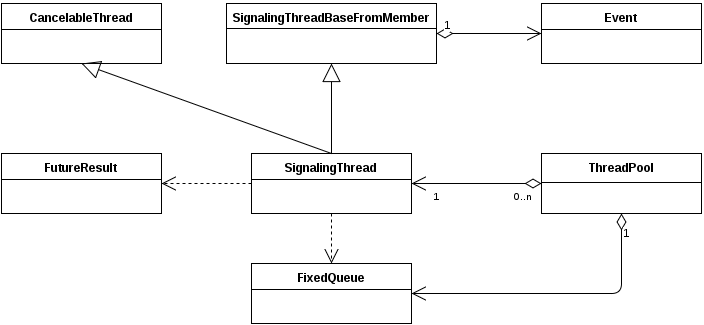
\includegraphics[width=1.0\textwidth]{img/class_diag.png}
  \caption{Дијаграм класа}
  \label{fig:klasa_dij}
\end{figure}


\begin{description}
	\item[Класа \texttt{Event}]\leavevmode
		\begin{itemize}
			\item[-] \texttt{void Signal(Sigval value = 1)} - емитује сигнал који је прослеђен као вредност \texttt{value}
			\item[-] \texttt{Sigval Value(bool block = false)} - враћа вредност сигнала који је емитован  
			\item[-] \texttt{static std::vector<std::size\_t> WaitForEvents(std::vector<Event::Pointer>\& events, const std::chrono::milliseconds \& waitMs = \{\}, bool block = true)} - омогућава ослушкивање више догаћаја истовремено
		\end{itemize}			
	\item[Класа \texttt{SignalingThread}]\leavevmode
		\begin{itemize}
			\item[-] \texttt{const Event::Pointer\& ShareEvent() const } - враћа дељени показивач на објекат догађаја 	
		\end{itemize}			
	\item[Класа \texttt{FixedQueue}]\leavevmode
		\begin{itemize}
			\item[-] \texttt{inline std::size\_t Size() const} - враћа број задатака у реду
			\item[-] \texttt{inline bool Empty() const} - испитује да ли је ред задатака 	празан	
			\item[-] \texttt{T* Pop()} - скида задатак са реда и враћа његов показивач
		\end{itemize}			
	\item[Класа \texttt{FutureResult}]\leavevmode
		\begin{itemize}
			\item[-] \texttt{void setResult(int val)} - иницијализује дељену вредност
			\item[-] \texttt{std::shared\_future<int>\& getSharedFuture()} - враћа референцу на објекат помоћу кога се може прочитати дељена вредност			
		\end{itemize}			
	\item[Класа \texttt{ThreadPool}]\leavevmode
		\begin{itemize}
			\item[-] \texttt{void Init(std::vector<std::function<int()>> \&\&tasks, uint64\_t num\_threads = std::thread::hardware\_concurrency() -1)} - поставља број нити, број задатака и конструише ред задатака	
			\item[-]\texttt{void StartWorkerThreads()} - покреће радне нити 			 		\item[-] \texttt{void StartControlThread()} - покреће контролну нит
			\item[-] \texttt{void Work()} - покреће базен нити
		\end{itemize}			
\end{description}


\section{Интеграција модула са системом LAV}

Паралелизација је имплементирана у контексту анализе наредби и функција модула који се верификује. 

\subsection{Паралелна анализа наредби}

Класа \texttt{LBlock} система LAV служи за рад са блоковима кода. Њена функција \texttt{CalculateConditions} конструише формуле које представљају услове исправности блока и позивају SMT решавач за сваку формулу. Модул за паралелизацију омогућава да се ови позиви решавача извршавају паралелно.

 За сваку формулу, услов исправности, унутар функције \texttt{CalculateConditions} конструише се функција која позива SMT решавач. Функција као резултат враћа индикатор да ли је услов исправности испуњен или не. Направљене функције се смештају у ред \texttt{FixedQueue} и прослеђују инстанци класе \texttt{ThreadPool} (базен нити). Базен нити прави радне нити и покреће их. Свака нит извршава једну по једну функцију, скидајући их са реда и обавештава базен нити о резултату извршавања. Уколико се наиђе на услов исправности који није задовољен, нема потребе испитивати остале услове јер се тада блок сматра неисправним. У контексту имплементације то значи да уколико нека функција врати индикатор да услов исправности није испуњен, нити могу престати са радом јер се задат блок означава као неисправан. Ако је приликом покретања система LAV (била) задата опција \texttt{-find-first-flawed} користи се понашање које је описано - прекидање у случају наиласка на неисправну наредбу. Ако та опција није присутна, онда се редом све испитује. Када све функције из реда заврше тако да су сви услови били задовољени, блок се сматра исправним и тако бива означен. 
 
 На слици \ref{fig:sekv_dij}  је приказан један могући сценарио. На почетку се врши конструкција и иницијализација свих потребних објеката. Базен нити конструише три радне нити које узимају задатке са реда. Нити  \texttt{SignalingThread1} прва узима задатак са реда, а након ње и \texttt{SignalingThread2} и обе почињу да их извршавају. Нит \texttt{SignalingThread1} прва завршава успешно, пре него што је нит \texttt{SignalingThread3} узела задатак са реда. Након тога обе нити,  \texttt{SignalingThread1} и  \texttt{SignalingThread3} покушају узети следећи задатак. Имајући у виду то да један ред задатака деле све нити, овај процес узимања задатака ће се извршити секвенцијално (користећи погодне функције из библиотеке  \texttt{<atomic>}) тако да нит \texttt{SignalingThread1} прва добија задатак са реда. Како нит  \texttt{SignalingThread1} наилази на услов исправности који није испуњен, шаље сигнал базену нити након чега остале нити бивају заустављене и систем LAV бива обавештен о неисправном резултату. Можемо приметити да је редослед акција прављења нити, узимање задатака са реда и брзина извршавања задатака у овом примеру конкретизован. Наравно, у општем случају тај редослед је произвољан и зависи од много фактора као што су специфичности оперативног система, сложеност задатака, број задатака у реду, и слично.  


\begin{figure}[!ht]
  \centering
  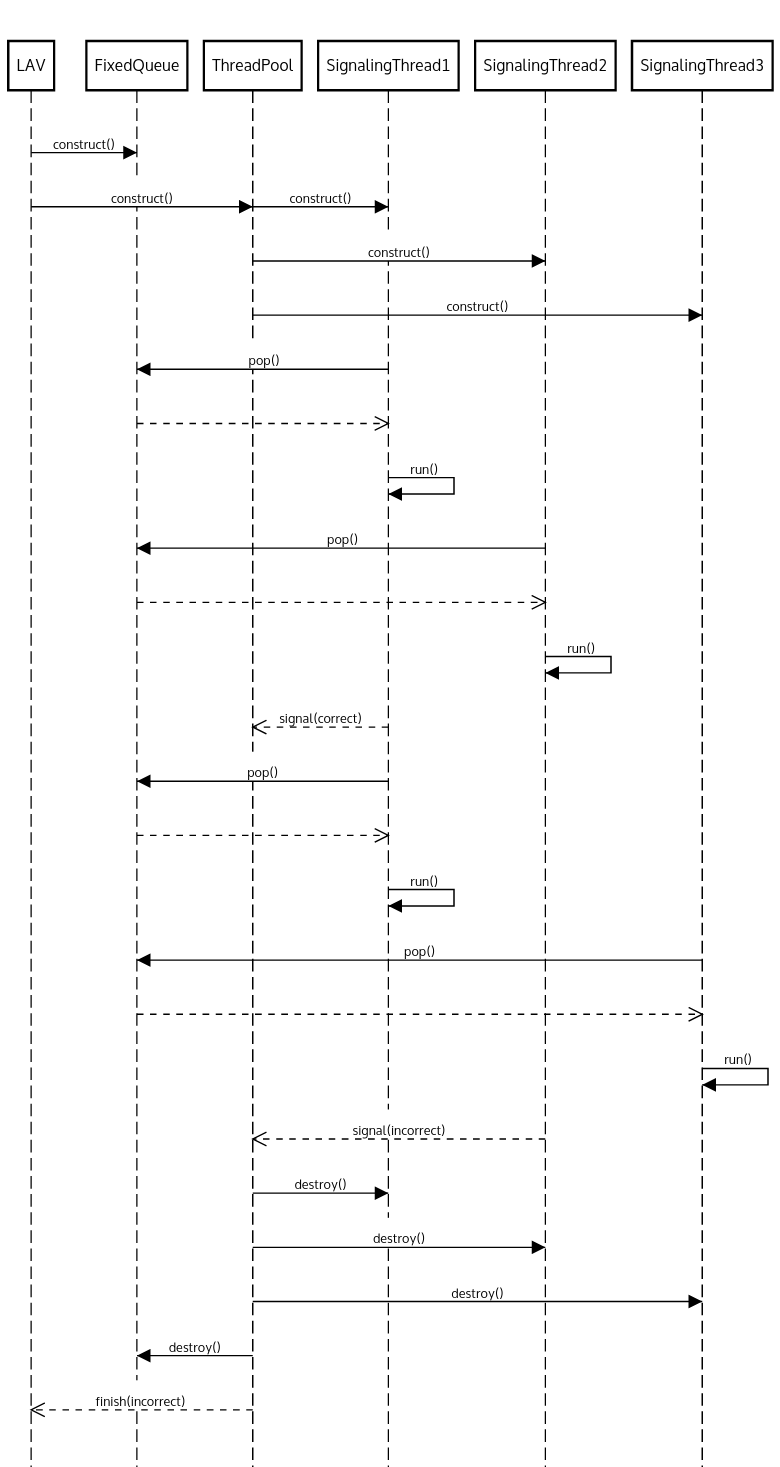
\includegraphics[width=0.8\textwidth]{img/seq_diag.png}
  \caption{Дијаграм тока извршавања}
  \label{fig:sekv_dij}
\end{figure}

\subsection{Паралелна анализа функција}

Анализа функција је имплементирана користећи исте механизме уз мале додатке због различитости проблема.   
 Класа \texttt{LModule} је одговорна за анализу функција једног модула. Функције могу зависити једне од других због чега је потребно чувати информације о резултату верификације сваке функције појединачно. Верификација модула почиње позивом метода \texttt{Run} класе \texttt{LModule} у оквиру кога се конструишу нити које анализирају функције тог модула. Класи \texttt{LModule} је додат низ објеката \texttt{FutureResult} за сваку функцију тог модула. Класа \texttt{FutureResult} представља структуру података унутар које се чува податак о завршетку верификације неке функције. Ова класа садржи објекат класе \texttt{std::promise}  који чува вредност (информацију о завршетку верификације) и објекат \texttt{std::future} помоћу кога нити приступају тој вредности. Свака нит има дељени показивач на низ објеката \texttt{FutureResult} тако да у сваком тренутку може погледати резултат верификације неке друге функције. Уколико се верификација тражене функције није завршила, тренутна нит ће сачекати на њен резултат позивом функције \texttt{wait} над објектом \texttt{std::future} за ту функцију. Када се верификација тражене функције заврши, резултат ће се уписати у њен објекат \texttt{std::promise} и функција \texttt{wait} ће завршити са чекањем. . Уколико је задата опција \texttt{-find-first-flawed} приликом наиласка на неисправну функцију, програм се означава неисправним, а остале нити се отказују чиме се верификација завршава. Иначе остале нити настављају са радом и тек након њиховог завршетка се верификација завршава.

\chapter{Експериментални резултати}

У наставку текста ће бити приказани резултати поређења модификованог система LAV са алатом CBMC. Корпуси на коме су тестирани алати, добијени резултати и све потребне скрипте за генерисање корпуса, покретање и чување резултата су јавно доступне и могу се пронаћи на адреси \url{http://argo.matf.bg.ac.rs/?content=lav}.


  \section{Архитектура рачунара}
  
  С обзиром на то да се рад заснива на паралелној импмементацији, експерименти су покретани на кластер рачунару са четрдесет и осам процесорских језгара, 94GB радне меморије и Ubuntu 16.04 оперативним системом. Максимално време извршавања програма је поставњено на 400 секунди. Време је мерено системским програмом \texttt{time}.
  
  \section{Опис корпуса}
  
  Експерименти су покретани на два корпуса, први демонстрира побољшање услед паралелне верификације блокова, а други демонстрира побољшање услед паралелне верификације функција програма.
  \subsection{Први корпус}
  
 Овај корпуса има за циљ да провери како се понаша паралелизације наредби услед великог броја сложених наредби у једном блоку. Корпус садржи двадесет програма писаних у програмском језику C. Сви програми у корпусу су конструисани на основу наведеног примера повећавајући број наредби. Програми су преведени у 32b и 64b формат како би се испитало да ли постоји значајна разлика у резултатима. Експерименти су показали да велика разлика не постоји, и због тога су се програми другог корпуса преводили само у 32b формат. \newpage

  
\begin{lstlisting}[basicstyle=\fontsize{4}{4}\selectfont,language=C,frame=single,caption=Пример програма,label=primer1]

int m(int a, int b, int c, int d) {

	// --- I skup ---
	// naredbe koje simuliraju slozena izracunavanja
	a = (b<<3)*((c>>2)/3);
	b = (a<<3)*((c>>2)/3);
	c = (b<<3)*((a>>2)/3);

	// --- II skup --- 
	// naredbe koje mogu dovesti do deljenja nulom
	a = b/c + b/a + c/(++b);
	b = a/d;
	
	return b;
}
\end{lstlisting}
 Програми су генерисани копирањем наредби из првог скупа одређен број пута. Понављање ових наредби симулира комплексна израчунавања која блок потенцијално може да садржи. За наредбе другог скупа је потребно утврдити да ли могу да доведу до дељења нулом. На пример, провера да ли су \texttt{a}, \texttt{b++} и \texttt{c} различите од нуле укључује комплексне формуле настале симболичким извршавањем наредби првог скупа, док је провера да ли је \texttt{d} различито од нуле једноставна.    


\subsection{Други корпус}

Наредни корпус се састоји од програма који садрже одређен број функција како би се демонстрирала верификација мало сложенијих програма. Корпус је подељен у две категорије од којих свака има две верзије и садржи 2000 програма писаних у програмском језику C. Програми овог корпуса не садрже наредбе неисправног дељења како би процес верификације обухватио пролазак кроз све путање програма (што је захтевније него у случају када се проналажењем грешке прекида извршавање).

\paragraph{Прва категорија} садржи програме са различитим бројем функција (од једне до педесет функција). Свака функција се састоји од одређеног број наредби које симулирају комплексна извршавања. Повећањем броја наредби отежава се провера коректности функција као и самог програма. Испитивање коректности потенцијално проблематичне наредбе дељења у првој верзији ове категорије не зависи од резултата претходних израчунавања, док у другој верзији зависи од резултата претходних израчунавања. Ово својство чини услове испитивања исправности лакшим у односу на програме друге верзије. Главна \texttt{main} функција позива све постојеће функције, због чега је за испитивање исправности програма потребно испитати исправност свих функција. Примери програма прве и друге верзије ове категорије се могу видети на сликама \ref{primer_nivo_1} и \ref{primer_nivo_1t}.

\paragraph{Друга категорија} се састоји од програма са различитим бројем функција које садрже позиве других функција. Повећањем дубине позива функција значајно се компликује испитивање коректности програма. Свака функција, као и у првој категорији, садржи наредбе које симулирају комплексна израчунавања и потенцијално проблематичне наредбе дељења. Такође, прва и друга, односно лакша и тежа, верзија ове категорије се разликују по сложености проблематичних наредби. Примери програма прве и друге верзије ове категорије се могу видети на сликама \ref{primer_nivo_2} и \ref{primer_nivo_2t}.
 
\begin{lstlisting}[basicstyle=\fontsize{4}{4}\selectfont,language=C,frame=single,caption=Пример програма прве категорије (прва верзија),label=primer_nivo_1]

int f1(int a, int b, int c) {

 // naredbe koje simuliraju slozena izracunavanja
 a = (b<<1)*((a>>1)/3);
 b = (a<<1)*((b>>1)/3);
  
 if(c!=0)
 //naredba deljenja za koju je potrebno utvrditi ispravnost
   return a/c;
   
 return a+b;
}

int main() {
 int a, b, c, r = 0;
 
 scanf("%d%d%d", &a, &b, &c);
 
 r += f1(a,b,c);
 
 return r;
}

\end{lstlisting}

\begin{lstlisting}[basicstyle=\fontsize{4}{4}\selectfont,language=C,frame=single,caption=Пример програма прве категорије (друга верзија),label=primer_nivo_1t]

int f1(int a, int b) {

 // naredbe koje simuliraju slozena izracunavanja
 a = (b<<1)*((a>>1)/3);
 b = (a<<1)*((b>>1)/3);
 
 if(b!=0)
 //naredba deljenja za koju je potrebno utvrditi ispravnost
   return a/b;
 
 return a+b;
}

int main() {
 int a, b, r = 0;
 
 scanf("%d%d", &a, &b);
 
 r += f1(a,b);

 return r;
}

\end{lstlisting}

\begin{lstlisting}[basicstyle=\fontsize{4}{4}\selectfont,language=C,frame=single,caption=Пример програма друге категорије (прва верзија),label=primer_nivo_2]

int _f1(int a, int b, int c) {

 // naredbe koje simuliraju slozena izracunavanja
 a = (b<<1)*((a>>1)/3);
 b = (a<<1)*((b>>1)/3);

 if(c!=0)
 //naredba deljenja za koju je potrebno utvrditi ispravnost
   return a/c;

 return a+b+c;
}

int f1(int a, int b, int c) {

 // naredbe koje simuliraju slozena izracunavanja
 a = (b<<1)*((a>>1)/3);
 b = (a<<1)*((b>>1)/3);

 if(c!=0)
 //naredba deljenja za koju je potrebno utvrditi ispravnost
 // i poziv druge funkcije 
   return a/c + _f1(a,b,c);

 return a+b+c;
}

int main() {

 int a, b, c, r = 0;

 scanf("%d%d%d", &a, &b, &c);

 r += f1(a,b,c);

 return r;
}


\end{lstlisting}



\begin{lstlisting}[basicstyle=\fontsize{4}{4}\selectfont,language=C,frame=single,caption=Пример програма друге категорије (друга верзија),label=primer_nivo_2t]
#include <stdio.h>

int _f1(int a, int b, int c) {

 // naredbe koje simuliraju slozena izracunavanja 
 a = (b<<1)*((a>>1)/3);
 b = (a<<1)*((b>>1)/3);
 
 if(b!=0)
 //naredba deljenja za koju je potrebno utvrditi ispravnost
   return a/b;
   
 return a+b+c;
}

int f1(int a, int b, int c) {

 // naredbe koje simuliraju slozena izracunavanja 
 a = (b<<1)*((a>>1)/3);
 b = (a<<1)*((b>>1)/3);
 
 if(b!=0)
 //naredba deljenja za koju je potrebno utvrditi ispravnost
 // i poziv druge funkcije 
   return a/b + _f1(a,b,c);
   
 return a+b+c;
}

int main() {
 int a, b, c, r = 0;
 
 scanf("%d%d%d", &a, &b, &c);
 
 r += f1(a,b,c);
 
 return r;
}


\end{lstlisting}



\subsection{Начини покретања}
%
%Приликом покретања алата LAV и CBMC над инстанцама програма првог и другог корпуса, коришћене су различите заставице и параметри како би се што боље демонстрирао рад алата и њихова ефикасност. У наставку ће бити описани начини покретања оба алата за програме из оба корпуса.
%
%\subsubsection{Први корпус}

Приликом покретања алата над инстанцама програма из овог корпуса алат LAV је покретан са опцијом заустављања приликом наиласка на прву невалидну наредбу, решавач који је коришћен је Z3. Број нити које користи LAV није експлицитно задат\footnote{То је број потребних нити односно број који је добијен као препорука оперативног система (и не мора представљати број физичких језгара на рачунару) уколико је потребно више нити него што систем дозвољава.}. Алат CBMC је покретан са параметром који испитује проблем дељења нулом. Име функције чију исправност је потребно испитати се експлицитно задаје заставицама \texttt{-starting-function=m} и \texttt{--function m} приликом покретања оба алата над програмима првог корпуса. Верификација инстанци другог корпуса подразумева испитивање исправности свих функција у програму и због тога није потребно задавање поменутих заставица јер је подразумевана почетна функција \texttt{main}.
\\ \\
Пример покретања LAV-а:
\\ \\
\texttt{./LAV 25\_lines.o -solver=Z3-BV-ARR-EUF -find-first-flawed -enable-parallel -starting-function=m}
\\ \\
Пример покретања CBMC-а:
\\ \\
\texttt{./CBMC --div-by-zero-check --32 --function m 25\_lines.c}

%\subsubsection{Други корпус}

  
 \section{Анализа резултата}
	У наставку ће бити изложена анализа резултата који су добијени покретањем алата LAV и CBMC над програмима из коришћених корпуса. 	
	
  Добијени резултати приликом верификације програма из првог корпуса се налазе у табели \ref{eksp_blok}, измерена времена су приказана у секундама. 
  
  Резултати показују да је време потребно алату CBMC за верификацију значајно веће од времена које је потребно алату LAV уз коришћење имплементиране паралелизације на нивоу блока. Разлог овоме је то што алат CBMC користи стандардне секвенцијалне технике испитивања исправности програма. Са повећањем броја наредби, повећавају се формуле које описују програм и чију задовољивост је потребно испитати, због чега се укупно време потребно за верификацију драстично увећава. Приметимо да је време потребно за верификацију програма који садржи двадесет и шест наредби користећи алат CBMC више него двоструко веће од времена које је потребно за верификацију програма од двадесет и пет наредби, док је разлика тих времена користећи алат LAV мала. Овакви резултати показују да паралелним испитивањем исправности наредби програма можемо драстично смањити укупно време које је потребно за верификацију и на тај начин унапредити постојеће алате.
  
\begin{table}
  \begin{tabularx}{1\textwidth}{|>{\setlength\hsize{1\hsize}\centering}X|>{\setlength\hsize{1\hsize}\centering}X|>{\setlength\hsize{1\hsize}\centering}X|>{\setlength\hsize{1\hsize}\centering}X|X|}
  \hline
  	\multirow{2}{*}{број наредби} & \multicolumn{2}{ c }{32b} &\multicolumn{2}{ | c | }{64b} 
	\\
	\cline{2-5}
	& LAV & CBMC & LAV & CBMC \\	
	\cline{1-5}
	12 & 0.08 & 0.72       & 0.07 & 0.82   \\	
	\cline{1-5}
	13 & 0.23 & 0.75       & 0.25 & 0.72   \\	
	\cline{1-5}
	14 & 0.38 & 0.93       & 0.08 & 0.93   \\	
	\cline{1-5}
	15 & 0.08 & 1.21       & 0.08 & 1.10   \\	
	\cline{1-5}
	16 & 0.27 & 1.42       & 0.09 & 1.46   \\	
	\cline{1-5}
	17 & 0.08 & 2.16       & 0.10 & 2.15   \\	
	\cline{1-5}
	18 & 0.10 & 3.08       & 0.23 & 3.05   \\	
	\cline{1-5}
	19 & 0.26 & 4.12       & 0.09 & 4.15   \\	
	\cline{1-5}
	20 & 0.11 & 7.80       & 0.21 & 7.93   \\	
	\cline{1-5}
	21 & 0.11 & 11.73      & 0.23 & 12.09  \\	
	\cline{1-5}
	22 & 0.22 & 16.50       & 0.23 & 17.28  \\	
	\cline{1-5}
	23 & 0.09 & 33.91      & 0.10 & 34.78  \\	
	\cline{1-5}
	24 & 0.11 & 52.50      & 0.10 & 53.46  \\	
	\cline{1-5}
	25 & 0.12 & 75.32      & 0.09 & 74.72  \\	
	\cline{1-5}
	26 & 0.11 & 157.01     & 0.10 & 154.87  \\	
	\cline{1-5}
	27 & 0.13 & 246.89     & 0.12 & 253.92  \\	
	\cline{1-5}
	28 & 0.12 & $\nearrow$ & 0.12 & $\nearrow$ \\	
	\cline{1-5}
	29 & 0.12 & $\nearrow$ & 0.13 & $\nearrow$ \\	
	\cline{1-5}
	30 & 0.14 & $\nearrow$ & 0.13 & $\nearrow$ \\	
	\cline{1-5}
	60 & 0.18 & $\nearrow$ & 0.20 & $\nearrow$ \\	
   \cline{1-5}
  \end{tabularx}

\caption[]{Експериментални резултати алата LAV и CBMC на првом корпусу {\label{eksp_blok}}}
\end{table}


  Резултати верификације програма из другог корпуса су приказани на графицима \ref{fig:nivo_1}, \ref{fig:nivo_1t}, \ref{fig:nivo_2} и \ref{fig:nivo_2t}. Алати су покретани са ограничењем времена на 400 секунди. Ради прегледности графика нису приказани сви резултати, већ су одабрани они резултати који показују одговарајући тренд раста.
  
  На графицима \ref{fig:nivo_1} и \ref{fig:nivo_2} се може видети да време потребно алату CBMC значајно расте услед повећања броја наредби у функцијама програма.  Такође можемо приметити да пораст времена зависи и од броја функција у програму. Алат CBMC достиже временско ограничење од 400 секунди већ на инстанци програма која садржи десет функција са шест наредби и још једним нивоом позива (тамно пLAVа испрекидана линија на графику \ref{fig:nivo_2}). 
  
  Такође, може се видети да време које је потребно алату LAV не расте великом брзином уколико повећавамо број наредби односно функција. Овакво понашање је резултат паралелног испитивања задовољивости SMT формула. Како проблематичне наредбе програма овог корпуса не зависе од резултата претходних сложених наредби, могуће је скоро па потпуно паралелизовати испитивање њихове коректности, и тиме умањити укупно потребно време. 
  
  Ако посматрамо однос времена које је утрошено коришћењем алата LAV и алата CBMC, можемо закључити да је паралелизација имплементирана унутар алата LAV значајно смањила (у неким случајевима за ред величина већи од $ 10^{2} $, љубичасте линије на графицима \ref{fig:nivo_1} и \ref{fig:nivo_2}) потребно време за верификацију програма из овог корпуса.
  
  На графицима \ref{fig:nivo_1t} и \ref{fig:nivo_2t} можемо да видимо измерена времена над инстанцама програма прве и друге категорије чија коректност се теже испитује. Ови програми, као што је описано у претходном поглављу, садрже проблематичне наредбе које зависе од резултата израчунавања претходних сложених наредби. Ово својство програма чини формуле чија се исправност испитује тежим, што резултује порастом времена потребног за верификацију. Али, и поред описаног ограничења, паралелизована верзија алата LAV потроши мању количину времена приликом верификације сложенијих програма у поређењу са алатом CBMC. Време потребно LAV-у за верификацију једноставнијих програма који садрже мањи број наредби је, у неким ситуацијама, веће од времена које је потребно алату CBMC. Ово показује да се паралелизација не исплати у свим ситуацијама јер конструисање контекста, прављење, покретање и синхронизација нити кошта односно троши одређено време.  
  
\begin{figure}[!ht]
  \centering
  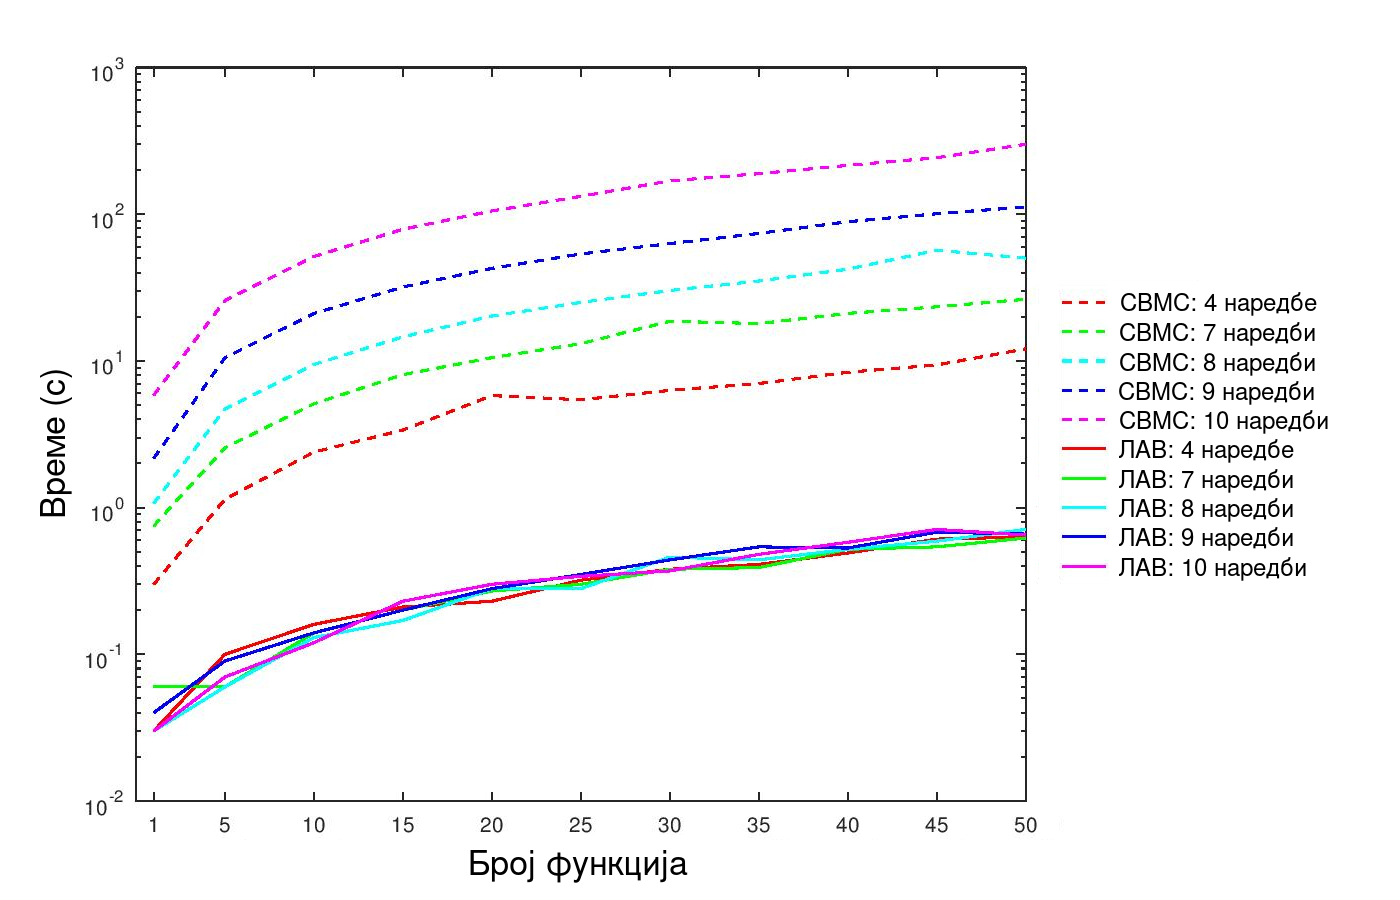
\includegraphics[scale=0.6]{img/nivo_1a.jpg}
  \caption{Прва категорија, лакша верзија}
  \label{fig:nivo_1}
\end{figure}

\begin{figure}[!ht]
  \centering
  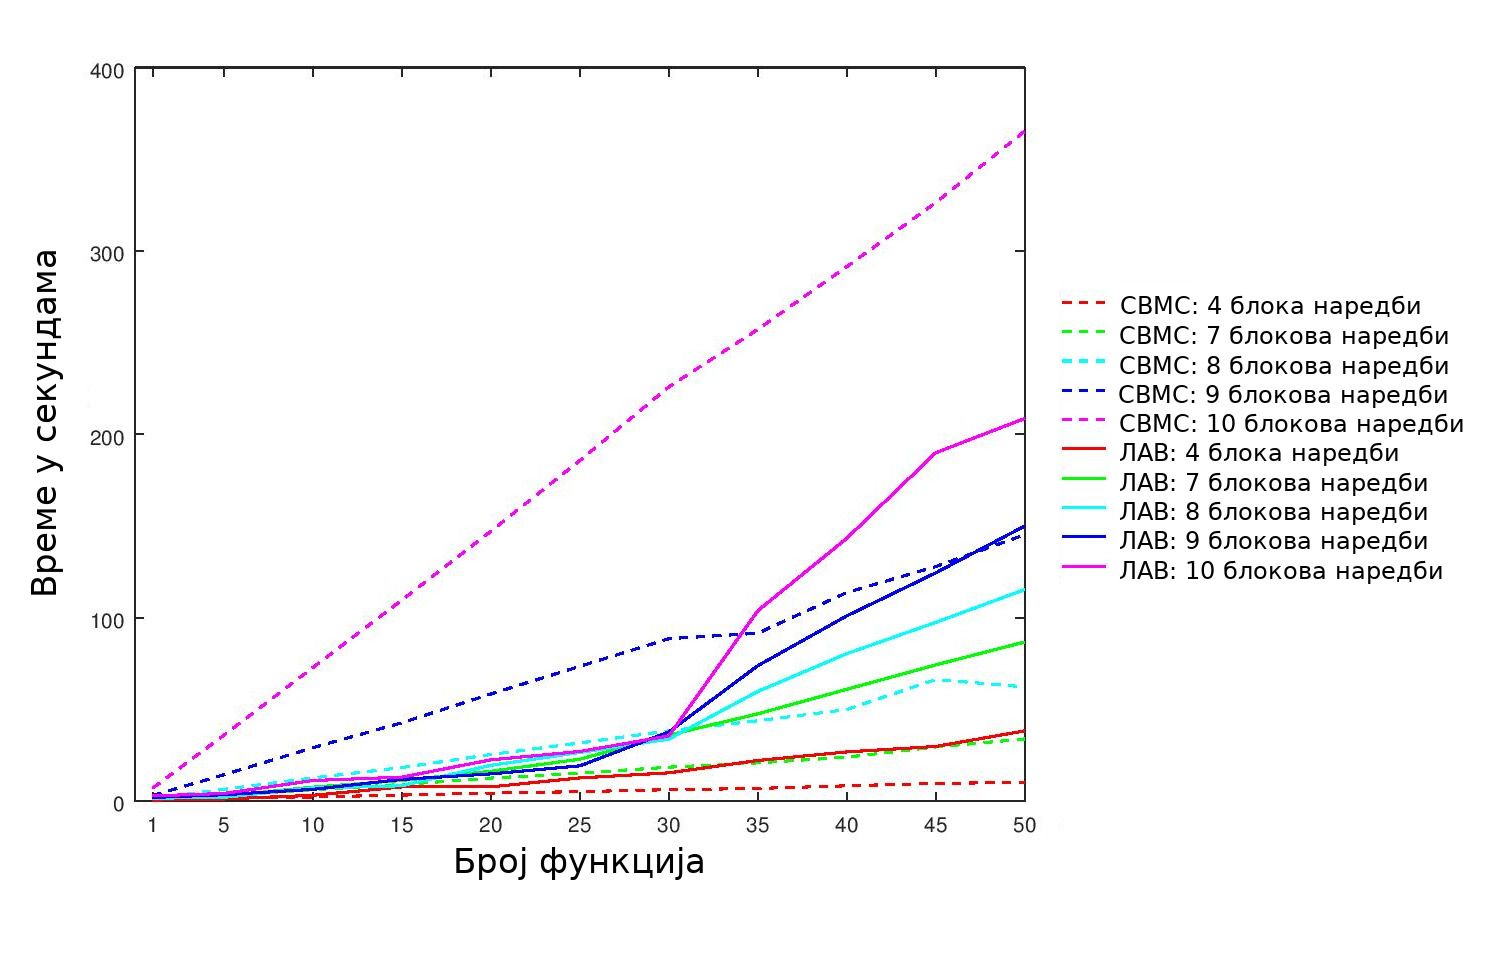
\includegraphics[scale=0.6]{img/nivo_1Ta.jpg}
  \caption{Прва категорија, тежа верзија}
  \label{fig:nivo_1t}
\end{figure}

\begin{figure}[!ht]
  \centering
  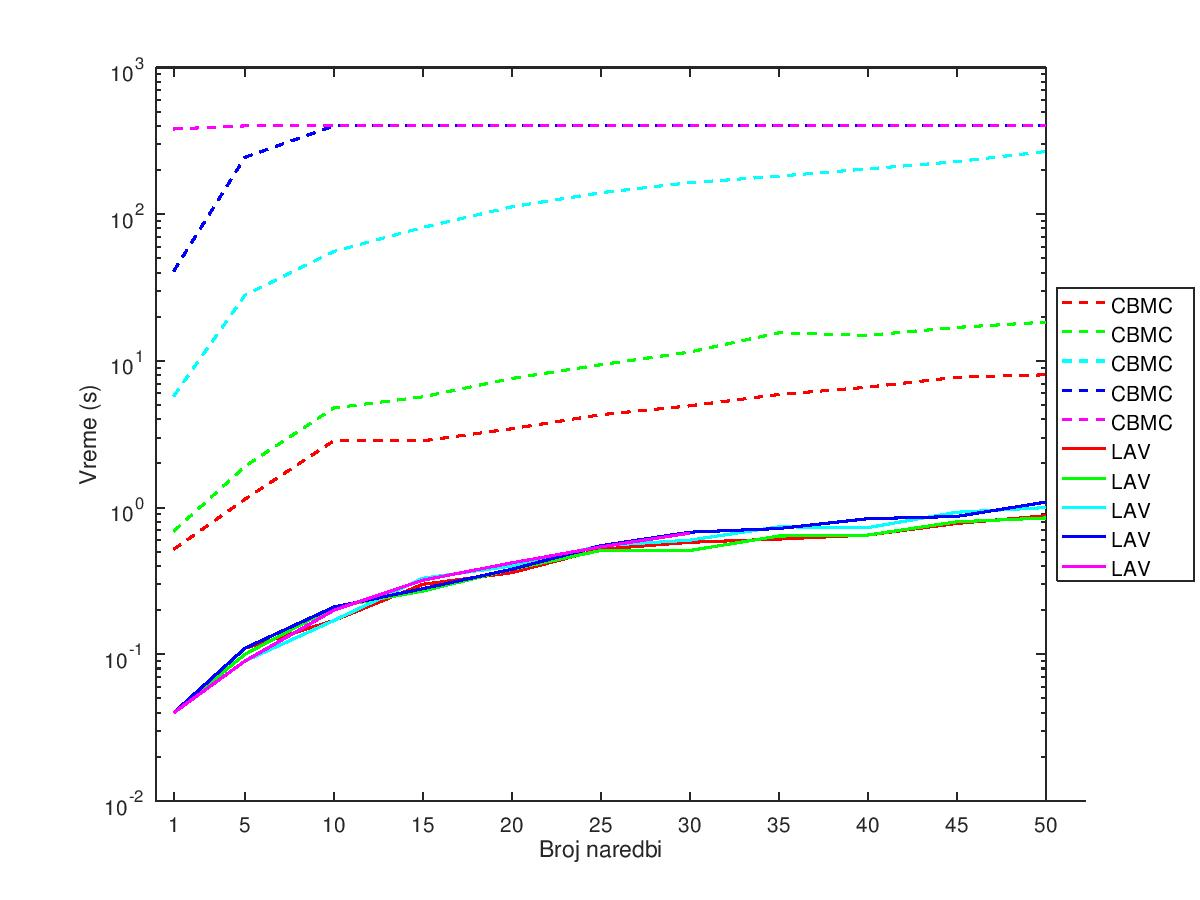
\includegraphics[scale=0.6]{img/nivo_2a.jpg}
  \caption{Друга категорија, лакша верзија}
  \label{fig:nivo_2}
\end{figure}

\begin{figure}[!ht]
  \centering
  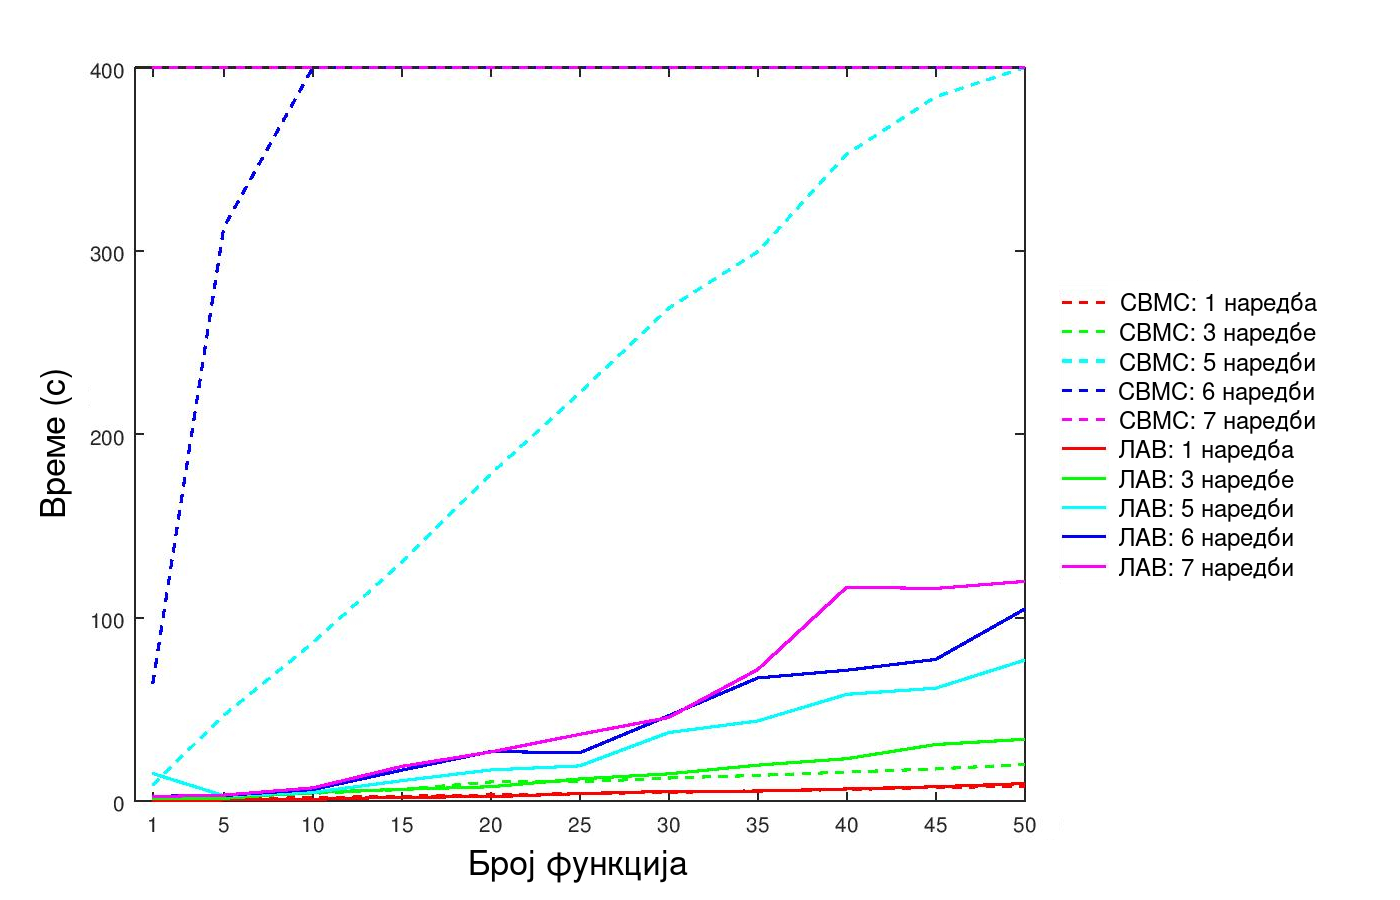
\includegraphics[scale=0.6]{img/nivo_2Ta.jpg}
  \caption{Друга категорија, тежа везија}
  \label{fig:nivo_2t}
\end{figure}


\chapter{Закључак} 

У овом раду разматран је проблем захтевности процеса верификације програма. Имплементирана је надоградња систему за верификацију LAV која паралелизује испитивање исправности софтвера на два нивоа, паралелном верификацијом блокова кода и паралелном верификацијом функција програма.

Унапређен алат LAV је тестиран на програмима из два корпуса. Инстанце програма првог корпуса су састављене са циљем да демонстрирају сложеност испитивања исправности блокова кода који садрже наредбе са комплексним израчунавањима. Програми другог корпуса садрже променљив број функција са различитим бројем наредби и дубином позива функција како би се показала временска захтевност верификације програма који садрже више од једне функције, што је најчешћи случај у данашњим софтверским решењима.

Изложени су експериментални резултати као и упоредна анализа алата LAV са сродним алатом CBMC. Резултати показују да за велике и комплексне програме предложено унапређење алата LAV значајно скраћује време потребно за утврђивање исправности програма. Приликом верификације једноставнијих програма дешава се да процес паралелизације захтева више времена него сама верификација, тако да је у тим случајевима није погодно користити.

Будућа истраживања на тему унапређења алата за верификацију би могла обухватити примене различитих метода машинског учења приликом одабира подскупа SMT формула чија задовољивост ће прва бити испитана. Још један смер побољшања може бити смањивање броја SMT формула као и њихово појединостављивање како би се редуковало време потребно за испитивање задовољивости.


\literatura
% ==============================================================================
% Završni deo teze i prilozi
\backmatter
\end{document}
